\documentclass[a4paper]{article}

%% Language and font encodings
\usepackage[english]{babel}
\usepackage[utf8x]{inputenc}
\usepackage[T1]{fontenc}
\usepackage{algpseudocode}
\usepackage{float}
\usepackage{booktabs}
\usepackage{amsmath}
\newtheorem{theorem}{Theorem}
%% Sets page size and margins
\usepackage[a4paper,top=3cm,bottom=2cm,left=3cm,right=3cm,marginparwidth=1.75cm]{geometry}

%% Useful packages
\usepackage{amsmath}
\usepackage{graphicx}
\usepackage{qtree}
\usepackage[colorinlistoftodos]{todonotes}
\usepackage[colorlinks=true, allcolors=blue]{hyperref}
\usepackage{tikz}
\usetikzlibrary{automata,positioning}
\usepackage{amsfonts}
\usepackage{amssymb}

\usepackage{forest}
\renewcommand{\rmdefault}{ptm}

\begin{document}
\section*{Count-min sketch: range queries}
Show and analyse the application of count-min sketch to range queries $(i,j)$ for computing  $\sum^j_{k=i} F[k]$. Hint: reduce the latter query to the estimate of just $t \leq 2\ log\ n$ counters $c_1,c_2,...,c_t$. Note that in order to obtain a probability at most $\delta$ of error (i.e. that $\sum^t_{l=1}c_l > \sum^j_{k=i}F[k] + 2\epsilon\ log\ n ||F||$), it does not suffices to say that it is at most $\delta$ the probability of error of each counter $c_l$: while each counter is still the actual wanted value plus the residual as before, it is better to consider the sum $V$ of these $t$ wanted values and the sum $X$ of these residuals, and apply Markov's inequality to $V$ and $X$ rather than on the individual counters.
\\
\\
\textbf{SOLUTION}
\\
\\
The proposed solution is based on a range tree, where we store a counter for each level of the tree. \\
At each level we keep a count-min sketch counter with parameter $\epsilon$ and $\delta$, fixed. Then every time an items $k$ arrives from the streaming we update the counter at each level $i$ of the tree with the following rule: $\frac{k}{2^{h-i}}$ where $h$ is the hight of the tree (i.e. $h=log_2$). Notice that at the leaf level we store the number as is it, and at each level we store the relative range. 
%\begin{figure}[H]
%\centering
%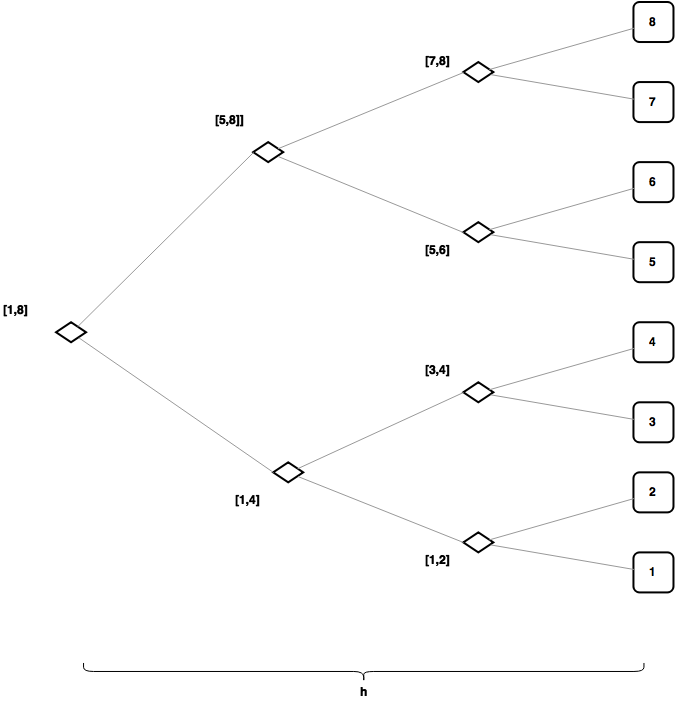
\includegraphics[scale=0.2]{tree.png}
%\end{figure}

\end{document}